\chapter{Pandas处理Excel}
与NumPy模块相比，pandas模块更擅长处理二维数据，其主要有\codeinline{Series}和\codeinline{DataFrame}两种数据结构。

\section{Excel文件操作}
\subsection{read\_excel 文件读取}
通过pandas模块可以从多种格式的数据文件中读取数据，也可以将处理后的数据写入这些文件中。
\begin{lstlisting}[style=demostyle,numbers=none]
import pandas as pd
df = pd.read_excel('xlsx文件')

# 或者
df = pd.read_excel('xlsx文件', sheetname='工作表名', endcoding='utf-8')
df = pd.read_excel('xlsx文件', sheetname=0, endcoding='utf-8',index_col=0)
## sheetname用于指定工作表，可以是工作表名称，也可以是数字（默认为0，即第1个工作表）
## encoding用于指定编码格式，默认为utf-8
## index_col用于指定索引列，默认为0，即第一列作为索引
\end{lstlisting}

除了读取Excel工作簿，pandas模块还可以读取CSV文件。
CSV文件本质上是一个文本文件，它仅存储数据，不能像Excel工作簿那样存储格式、公式、宏等信息，
所以所占存储空间通常较小。
CSV文件一般用逗号分隔一系列值，既可以用Excel打开，也可以用文本编辑器（如“记事本”）打开。
\begin{lstlisting}[style=demostyle,numbers=none]
# 读取csv文件
df = pd.read_csv('csv文件')

# 或者
data = pd.read_csv('csv文件.csv', delimiter=',', encoding='utf-8')
## delimiter用于指定分隔符，默认为逗号
## encoding用于指定编码格式，默认为utf-8
\end{lstlisting}

\subsection{DataFrame.to\_excel 文件写入}
\begin{lstlisting}[style=demostyle,numbers=none]
import pandas as pd   

DataFrame.to_excel('xlsx文件')

# 或者
DataFrame.to_excel('xlsx文件', sheet_name='工作表名', encoding='utf-8', index=False)
## sheet_name用于指定工作表名称，默认为'Sheet1'
## encoding用于指定编码格式，默认为utf-8
## index=False用于不写入索引列

DataFrame.to_excel('xlsx文件',index=['A','B','C'])
\end{lstlisting}        

\begin{figure}[htbp]
\centering
\begin{minipage}[t]{0.3\textwidth}
  \centering
  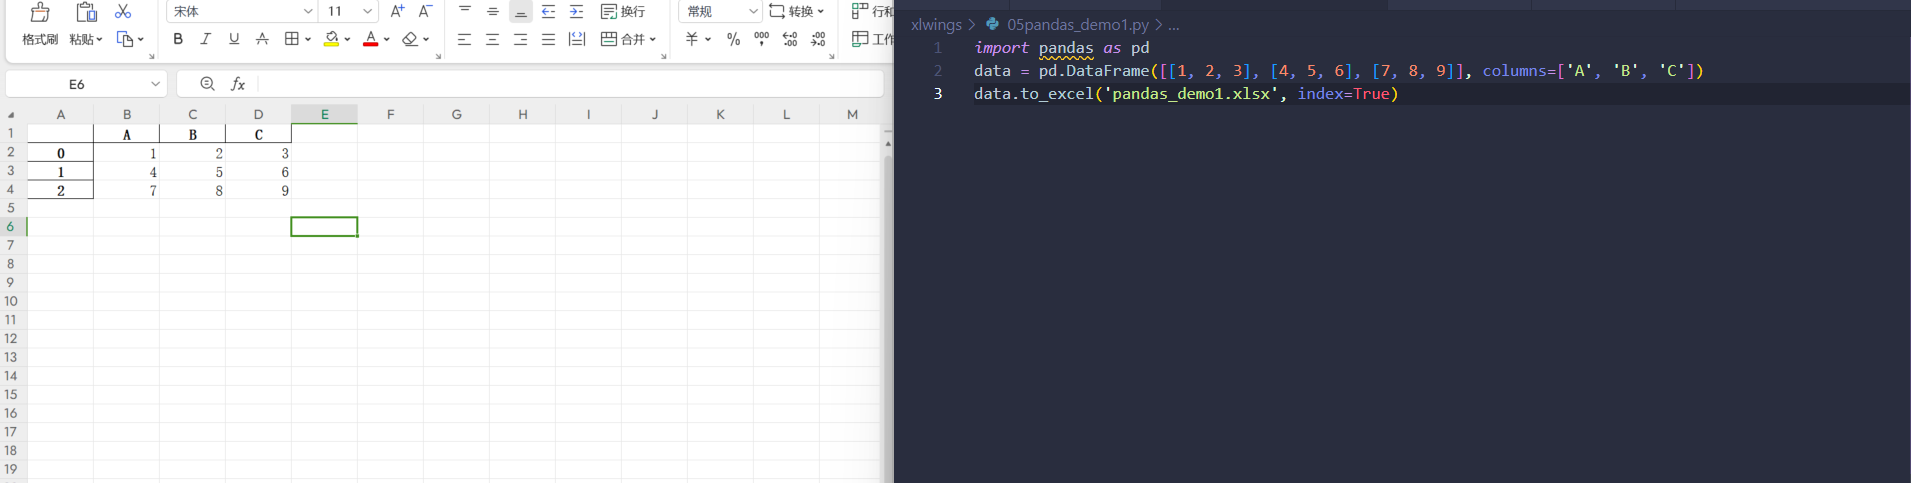
\includegraphics[width=0.7\linewidth]{part/自动化/办公自动化/pic/excel/pandas/pandas写入xlsx写入index.png}
  \caption{index=True}
\end{minipage}
\hspace{0.1\textwidth} % 调整这里的参数来改变图片之间的空隙
\begin{minipage}[t]{0.3\textwidth}
  \centering
  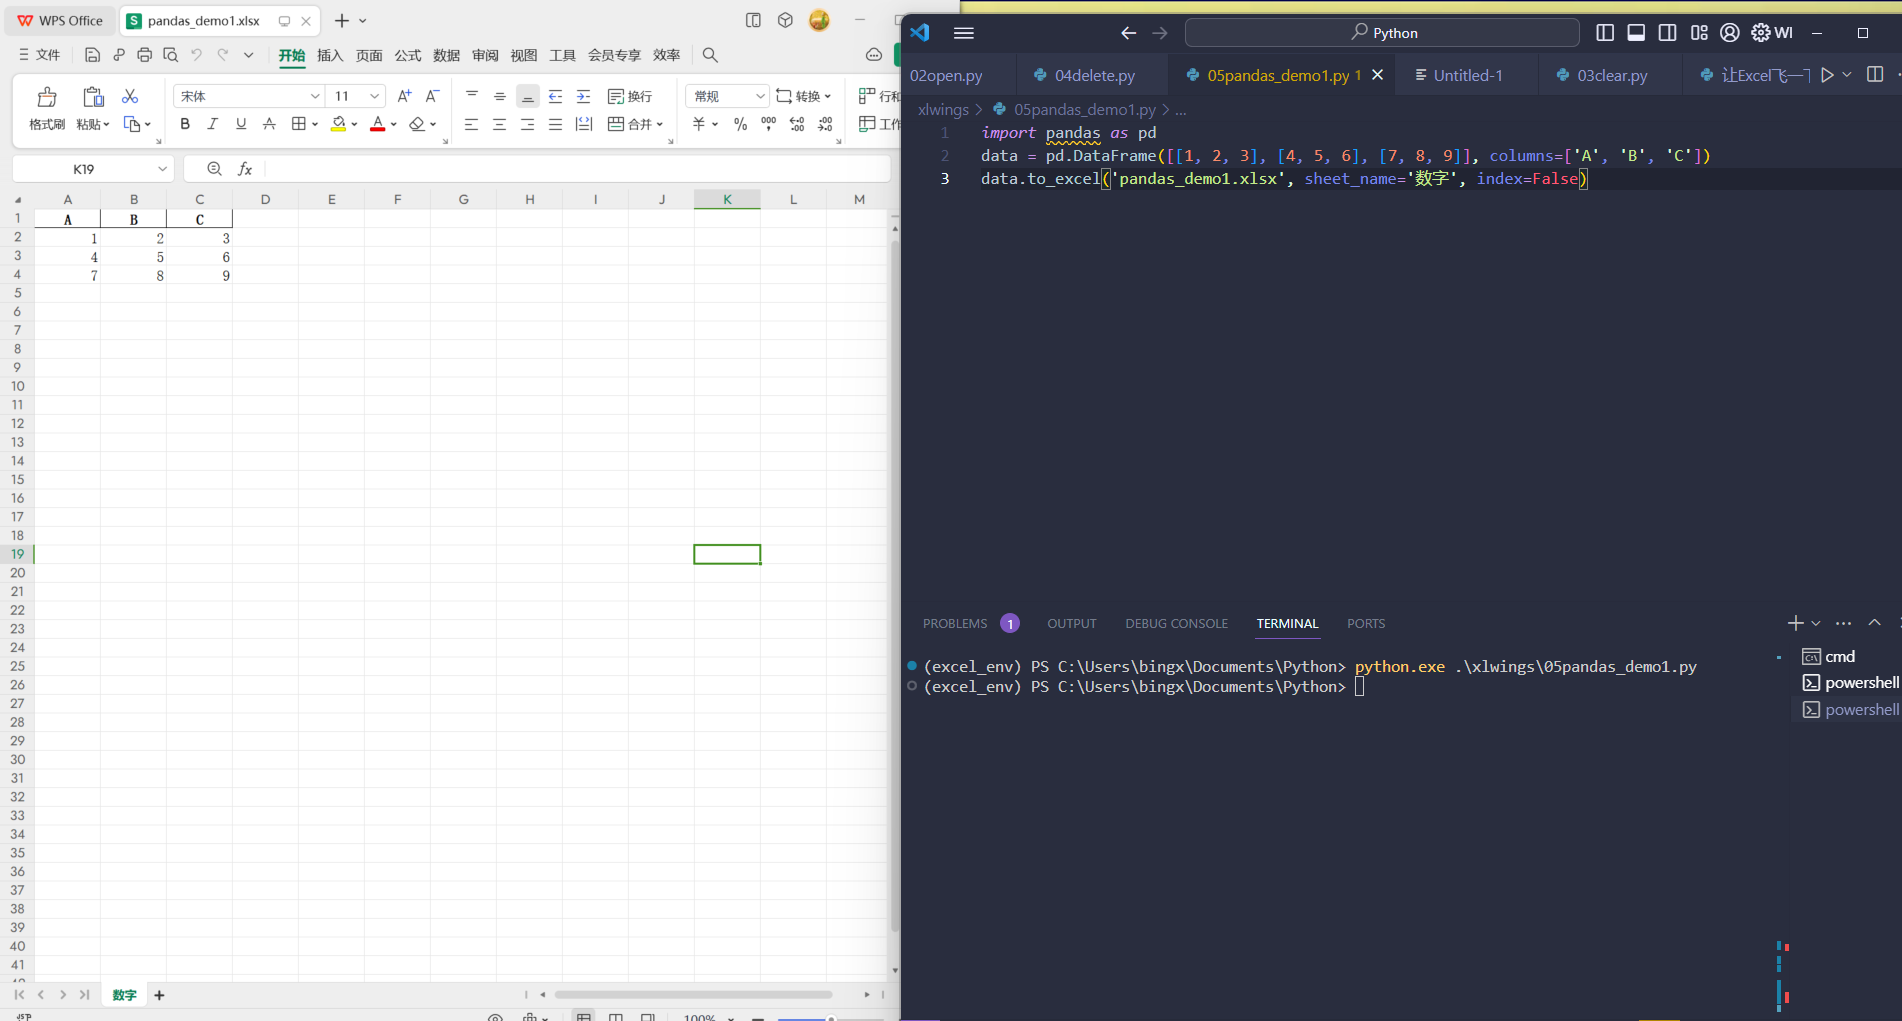
\includegraphics[width=0.7\linewidth]{part/自动化/办公自动化/pic/excel/pandas/pandas写入xlsx指定sheet名不写入index.png}
  \caption{sheetname='数字',index=False}
\end{minipage}
\caption{pandas写入Excel}
\end{figure}

\section{Sheet工作表(sheet)}
\subsection{读取工作表(sheet)}
\begin{lstlisting}[style=demostyle,numbers=none]
# 读取工作表(sheet)
df = pd.read_excel('xlsx文件', sheet_name='工作表名')
\end{lstlisting}

\subsection{写入工作表(sheet)}
\begin{lstlisting}[style=demostyle,numbers=none]
# 写入工作表(sheet)
df.to_excel('xlsx文件', sheet_name='工作表名')

# 写入多个 Sheet：pd.ExcelWriter
with pd.ExcelWriter('xlsx文件') as writer:
    df1.to_excel(writer, sheet_name='Sheet1')
    df2.to_excel(writer, sheet_name='Sheet2')
\end{lstlisting}

\section{Cell单元格}
Pandas \textcolor{red}{\textbf{不直接}}提供单元格级别操作，但可以通过 DataFrame 来间接实现：
\subsection{获取单元格}
\subsubsection{按行/列索引获取单元格}
\begin{enumerate}[label=\arabic*)]
    \item \codeinline{df['列名']}: 获取整列数据
    \item \codeinline{df[['列名1', '列名2']]}: 获取多列数据
    \item \codeinline{df.iloc[行索引]}: 获取整行数据
    \item \codeinline{df.iloc[[行索引1, 行索引2]]}: 获取多行数据
    \item \codeinline{df.head(n)}: 获取前n行数据
\end{enumerate}

\subsubsection{按区块获取单元格}
\begin{enumerate}[label=\arabic*)]
    \item \codeinline{df['列名'][行索引]}: 先根据列名获取列数据，再根据行索引获取单元格数据
    \item \codeinline{df.iloc[行索引][列索引]}: 先根据行索引获取行数据，再根据列索引获取单元格数据
\end{enumerate}

\subsection{数据筛选}
\begin{lstlisting}[style=demostyle,numbers=none]
import pandas as pd  
df = pd.read_excel('xlsx文件')
df[df['列名'] > 0] # 筛选列名大于0的行  

# 多条件筛选
df[(df['列名1'] > 0) & (df['列名2'] > 0)] # 筛选列名1和列名2都大于0的行
\end{lstlisting}

\subsection{sort\_values 排序}  
\begin{lstlisting}[style=demostyle,numbers=none]
import pandas as pd  
df = pd.read_excel('xlsx文件')
df.sort_values('列名', ascending=True) # 升序排序
df.sort_values('列名', ascending=False) # 降序排序
\end{lstlisting}

\subsection{数据运算}
\begin{lstlisting}[style=demostyle,numbers=none]
import pandas as pd  
df = pd.read_excel('xlsx文件')
df['新的列名'] = df['列名1'] + df['列名2'] # 列名1和列名2相加
df['新的列名'] = df['列名1'] - df['列名2'] # 列名1和列名2相减
df['新的列名'] = df['列名1'] * df['列名2'] # 列名1和列名2相乘
df['新的列名'] = df['列名1'] / df['列名2'] # 列名1和列名2相除
\end{lstlisting}

\subsection{drop 删除行/列}
\begin{lstlisting}[style=demostyle,numbers=none]
import pandas as pd  
df = pd.read_excel('xlsx文件')
df.drop(0) # 删除第一行
df.drop([0, 1]) # 删除第一行和第二行
df.drop('列名') # 删除列名对应的列
\end{lstlisting}


\subsection{数据表的拼接}
\subsubsection{merge 拼接}
\codeinline{merge()}函数可以根据一个或多个同名的列将不同数据表中的行连接起来。
\begin{lstlisting}[style=demostyle,numbers=none]
pd.merge(left, right, how='inner', on='key_column')
# left和right是要连接的两个数据表
# how用于指定连接方式，inner（内连接）、outer（外连接）、left（左连接）、right（右连接）
# on用于指定连接的列名
\end{lstlisting}

\begin{lstlisting}[style=pythonstyle,numbers=left]
import pandas as pd

# 两个数据表
df1 = pd.DataFrame({'ID': [1, 2, 3], 'Name': ['Alice', 'Bob', 'Charlie']})
df2 = pd.DataFrame({'ID': [2, 3, 4], 'Score': [85, 90, 95]})
print("df1:{}\n".format(df1))
print("df2:{}\n".format(df2))


# 按 ID 列进行内连接
result = pd.merge(df1, df2, how='inner', on='ID')
print(result)
\end{lstlisting}
\begin{lstlisting}[style=demostyle,numbers=none]
df1:   ID     Name
0   1    Alice
1   2      Bob
2   3  Charlie

df2:   ID  Score
0   2     85
1   3     90
2   4     95

   ID     Name  Score
0   2      Bob     85
1   3  Charlie     90
\end{lstlisting}

\subsubsection{concat 全连接}
\codeinline{concat()}函数使用全连接（UNION ALL）方式完成拼接，
它不需要对齐，而是直接进行合并，
即不需要两个表有相同的列或索引，只是把数据整合到一起。

因此，该函数没有参数\codeinline{how}和\codeinline{on}，而是用参数\codeinline{axis}指定连接的轴向。
该参数默认值为0，指按行方向连接（纵向拼接）。

\begin{lstlisting}[style=demostyle,numbers=none]
pd.concat([df1, df2], axis=0)
# axis=0表示按行方向连接（纵向拼接）
# axis=1表示按列方向连接（横向拼接）
\end{lstlisting}

\begin{lstlisting}[style=pythonstyle,numbers=left]
import pandas as pd
# 两个数据表
df1 = pd.DataFrame({'A': [1, 2], 'B': [3, 4]})
df2 = pd.DataFrame({'A': [5, 6], 'B': [7, 8]})
print("df1:{}\n".format(df1))
print("df2:{}\n".format(df2))

# 按行拼接
result_row = pd.concat([df1, df2], axis=0, ignore_index=True)

# 按列拼接
result_col = pd.concat([df1, df2], axis=1)
print("按行拼接:")
print(result_row)
print("\n按列拼接:")
print(result_col)
\end{lstlisting}
\begin{lstlisting}[style=demostyle,numbers=none]
df1:   A  B
0  1  3
1  2  4

df2:   A  B
0  5  7
1  6  8

按行拼接:
   A  B
0  1  3
1  2  4
2  5  7
3  6  8

按列拼接:
   A  B  A  B
0  1  3  5  7
1  2  4  6  8
\end{lstlisting}


\subsubsection{append 纵向拼接}
\codeinline{append()} 是 \codeinline{concat()} 的简化版本，通常用于按行追加数据(\codeinline{axis=0})。

\begin{lstlisting}[style=demostyle,numbers=none]
df1.append(df2, ignore_index=True)
# ignore_index=True表示忽略原索引，生成新的索引
\end{lstlisting}
\begin{lstlisting}[style=pythonstyle,numbers=left]
import pandas as pd
# 两个数据表
df1 = pd.DataFrame({'A': [1, 2], 'B': [3, 4]})
df2 = pd.DataFrame({'A': [5, 6], 'B': [7, 8]})
print("df1:{}\n".format(df1))
print("df2:{}\n".format(df2))
result = df1._append(df2, ignore_index=True)
print(result)
result = df1._append(df2, ignore_index=False)
print(result)
\end{lstlisting}
\begin{lstlisting}[style=demostyle,numbers=none]
df1:   A  B
0  1  3
1  2  4

df2:   A  B
0  5  7
1  6  8

   A  B
0  1  3
1  2  4
2  5  7
3  6  8

   A  B
0  1  3
1  2  4
0  5  7
1  6  8
\end{lstlisting}
